\documentclass{article}

\usepackage[utf8]{inputenc}
\usepackage[T1]{fontenc}
\usepackage{geometry}
\usepackage{xcolor}
\usepackage{graphicx}
\usepackage{subcaption}
\usepackage{verbatim}
\usepackage{amsmath,amssymb}
\usepackage{amstext}
\usepackage{amsthm}
\usepackage{steinmetz}
\usepackage{stackrel}
\usepackage{mathtools}
\newcommand{\angstrom}{\text{\normalfont\AA}}

\geometry{a4paper}

\usepackage[english]{babel}
\frenchspacing

\title{Report: adder and subtractor}
\author{Lorenzo Ramella, Alessandro Matteo Rossi, Marco Tambini}
\date{\today}

\begin{document}
\maketitle

\tableofcontents

\section{Basics concepts}

To make calculations, a circuit needs to be able to perform logical operations. In particular, we usually use boolean algebra in digital electronics. 

\vspace{3mm}

To be able to create a circuit like this, first of all, we need to define the various components.
The number 0 and 1 have to be properties of an electric circuit that can be "moved"; the easiest waof this proprieties to use is the voltage so we can assign the number 0 to a low voltage and the number 1 to a high voltage. 

\vspace{3mm}

For example, if we define $0\,\textrm{V}$ as low, negative or 0 and $5\,\textrm{V}$ as high, positive or 1, we can define a threshold voltage exactly in the middle, so that any voltage under $2.5\,\textrm{V}$ will be considered 0, and any voltage above it will be considered 1.

\vspace{3mm}

Once 1 and 0 are defined, we need to define the operations that can be performed:

\begin{itemize}
\item $"!"$ is the negation, and it can be represented by a NOT gate.
\item $"+"$ is the addition, and it can be represented by a OR gate.
\item $"*"$ is the multiplication, and it can be represented by an AND gate.
\end{itemize}

\section{Logic gates}

When we talk about a logic gate, we are talking about a circuit that can take a certain number of inputs and give a single output, depending on the input received; the output needs to be readable by another logic gate of the same family.

The main logic gates are the following:

\begin{figure}[h]

    \centering
    \begin{subfigure}{.49\textwidth}
        \centering
        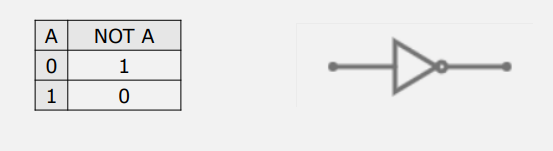
\includegraphics[width=\linewidth]{IM_NOT.PNG}
        \caption{NOT gate}
        \label{NOT}
    \end{subfigure}
    \hfill
    \begin{subfigure}{.49\textwidth}
        \centering
        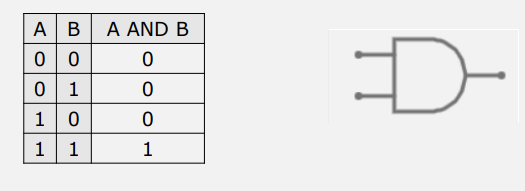
\includegraphics[width=\linewidth]{IM_AND.PNG}
        \caption{AND gate}
        \label{AND}        
    \end{subfigure}
    
    \centering
    \begin{subfigure}{.49\textwidth}
        \centering
        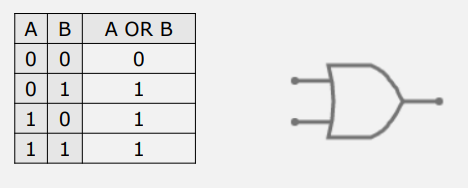
\includegraphics[width=\linewidth]{IM_OR.PNG}
        \caption{OR gate}
        \label{OR}
    \end{subfigure}
    \hfill
    \begin{subfigure}{.49\textwidth}
        \centering
        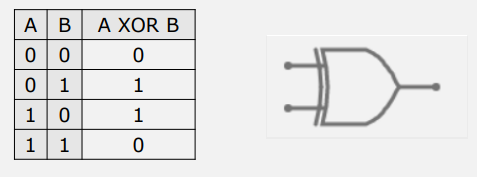
\includegraphics[width=\linewidth]{IM_XOR.PNG}
        \caption{XOR gate}
        \label{XOR}        
    \end{subfigure}
    
    \centering
    \begin{subfigure}{.49\textwidth}
        \centering
        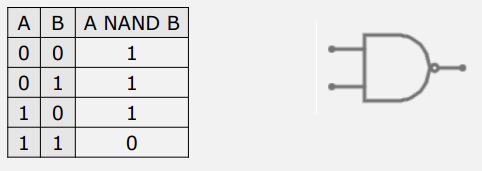
\includegraphics[width=\linewidth]{IM_NAND.PNG}
        \caption{NAND gate}
        \label{NAND}
    \end{subfigure}
    \hfill
    \begin{subfigure}{.49\textwidth}
        \centering
        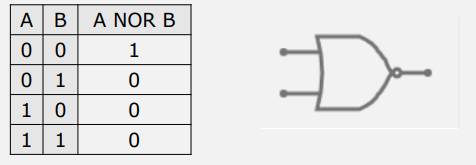
\includegraphics[width=\linewidth]{IM_NOR.PNG}
        \caption{NOR gate}
        \label{NOR}        
    \end{subfigure}
    
    \centering
    \begin{subfigure}{.49\textwidth}
        \centering
        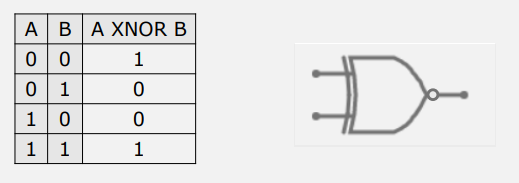
\includegraphics[width=\linewidth]{IM_XNOR.PNG}
        \caption{XNOR gate}
        \label{XNOR}
    \end{subfigure}
\label{Logic_Gates}
\caption{Image of the main logic gates used in digital electronics}
\end{figure}


\subsection{N-mos}

To crete the logic gate we need to first know how to use a MOSFET. In our case we used only N-MOS. 

\vspace{3mm}

The N-MOS is a transistor that get in input a gate voltage, a drain voltage, a source voltage and a body voltage; in most cases the source and the body are internally connected since the body needs to be at the lowest voltage and the source is usually at mass.

When a positive voltage is aplied between the drain and source a deplition layer block the passage of current is formed and there is no passage of current. 
If we then start aplying a positive voltage between gate and body the electron will start "balancing" the gaps in the P substrate but there will still be no passage of current. 

After $V_{GS}$ surpass a threshold voltage the current will start to flow from drain to source. At the start the ratio between the current and $V_{DS}$ is linear but, when $V_{DS}$ is big enough, the ratio stop to grow and become almost linear as seen in Immage %number of immage
and we find ourself in the region of saturation.

\vspace{3mm}

We didn't really need to differentiate in linear section and saturation section of the N-MOS since what we will check is the voltage at the drain of the N-MOS for our gate.
The threshold voltage vary between transistor and usually go from $0.5V$ to $5V$. 
The transistor we used is the $IRF822$ and we found in lag that the threshold voltage is approssimatively %nV
, we decided to use $5V$ for $V_{GS}$ to make, as we will see later, input and output aproximativaly the same.



\subsection{NOT gate}

The easiest gate to realizeis the not gate; we remember that he NOT gate negate the input and so work with a single input.

To realize it we need a resistance high enough and the N-MOS as seen in Immage% number of immage

%immage of the NOT gate

\vspace{3mm} %to remove after the immage is added

When the input is 0 the N-MOS will not let the current flow and, thanks to ohm first law, we know that the voltage drop on the extreme of the resistance should be 0 getting the same voltage of the alimentation. 

The output readed  will be around $5V$ so we got a 1

When the input is 1 the N-MOS will let the current flow and offer a small resistance; since there is a much bigger resistance before the N-MOS almost all the voltage drop will happen on the former and the voltage on the drain will be almost zero.

The output readed will be around $0V$ so we got a 0

\vspace{3mm}

with this configuration we find out that, with high frequencies, the signal will not be properly negated and will instead be like in Immage% number of immage Inverter N-MOS a carico resistivo
and instead pass almost all the time in a 0 state. 

A solution we could use is a combination of N-MOS and P-MOS but, since our calculator sholdn't have to work at such frequencies, we dismised this problem.

\vspace{3mm}

For the immage of the NOT gate and some result we got in lab check the end of the report at %number of appendix chapter subsection not gate



\subsection{NOR gate}

Once we ralized the NOT gate we proceeded to realize the NOR gate since, as we will talk later in %number of paragraph "other gate"
, the NOR and the NAND gate are both functionally complete.

The NOR gate is composed, as seen in Immage% number of immage
, by two NOT gate shortcircuited at the output.

%immage of the NOR gate

\vspace{3mm} %to remove after the immage is added

When both output are 0 the two N-MOS will not let any current pass and; just like in the NOT gate, the output will be 1.

When one or both the input are 1 the N-MOS will let the current flow and there will be a voltage drop at the extreme of the resistance; just like in the NOT gate the output will be 0.

The role of the short circuit is to make sure that doesn't matter which of the input is positive since the current will surely pass throught the "open" N-MOS.

\vspace{3mm}

For the immage of the NOR gate and some result we got in lab check the end of the report at %number of appendix chapter subsection nor gate

\subsection{NAND gate}

Like we said for the NOR gate the NAND gate is also functionally complete but has the advantage of not needing the shortcircuit and one of the resistances needed by the NOR gate making it slightly cheaper than the NOR gate. 

To create it we put in series first the resistance and after the two N-MOS joining the source of the first and the drain of the second as seen in Immage%number of immage
.

\vspace{3mm} %as always to remove after the immage is added

In case both input are 1 the current will be able to flow and, the output will be 0

When even one of the input is 0 one of the N-MOS will be "closed" and, since the current cannot pass, the output will be 1.

\vspace{3mm}

For the immage of the NAND gate and some result we got in lab check the end of the report at %number of appendix chapter subsection nand gate



\subsection{Other gate}

The propriety of the NOR and NAND gate of being functionally complete means that all the other logic gate can be recreated by that one. 

Since we already created the NOT gate we don't really care about how it's done but in case check Immage %number of immage about functional completness of NAND and NOR in appendix 
in %subchapter of appendix with the immage above
. 

The gate needed for the calculator are: 

\begin{itemize}
\item The AND gate mady by the NAND gate where the output is negated by a NOT as see in in Immage % number of immage AND
\item The OR gate made by the NOR gate where the output is negated by a NOT as seen in Immage % number of immage OR
\item The XOR gate made by four NAND gate put in the configuration of Immage % number of immage XOR
\end{itemize}

%immage of the NNAND, NNOR and XOR gate 

\subsection{Bistable circuit}

For the 16-bit calculator of wich we will talk in section %section of the simulated calculator
we also needed to be able to store information. 

For a circuit to be ablo to work as a memory it need to be able to get an input and keep it even after it has ended. Since the memory should be both modificable and readable it need a second input to clear it and should be ablo to give an output.

\vspace{3mm}

The circuit that correspond to the memory that we need is the bistable circuit also known as flip-flop.
The flip-flop can be created by both NOR gate and NAND gate but, since the NAND gate are less expensive, we decided to use those in our project with the knowledge that the input should be negated for it to work.

We report in Table 1 and Immage %number of the immage of the flip flop
the flip flop we created and his truth table.

%immage of the flip flop

\begin{table}[h!]
\centering
\begin{tabular}{ | c | c  c  c | c  c |}
\hline
 \# & $Set$ & $Clear$ & $Old Q$ & $New Q$ & $New Q'$\\
\hline
 \ 1 & 0 & 0 & 0 & 1 & 1 \\ 
 \ 2 & 0 & 0 & 1 & 1 & 1 \\
\hline 
 \ 3 & 0 & 1 & 0 & 1 & 0 \\ 
 \ 4 & 0 & 1 & 1 & 1 & 0 \\ 
 \ 5 & 1 & 0 & 0 & 0 & 1 \\
 \ 6 & 1 & 0 & 1 & 0 & 1 \\
\hline
 \ 7 & 1 & 1 & 0 & 0 & 1 \\
 \ 8 & 1 & 1 & 1 & 1 & 0 \\ 
\hline
\end{tabular}
\caption{Truth table of the flip-flop. As seen the line 1 and 2 are not ideal for the storage of memory. 3, 4, 5 and 6 are condition where one input is given. 7 and 8 are condition where data is stored.}
\label{table:1}
\end{table}




\section{16-bit calculator}



\subsection{Input with 16-bit}

One of the problem that arise when we want to use more memory space is an increase in complexity; this one make the circuit more expensive and also take space that could be used for other pourpose. 

While in a small scale we could use a 2-bit priority encoder for our project on the simulator we wanted to create a calculator tht could operate with 16 bit in input and give an output just as big, excluding sign bit; to do that a priority encoder would be inpractical and unnecessarely more complex.
Another problem that would araise in that of the phisical input since  priority encoder would require as many input as the number of decimal number we want.

\vspace{3mm}

To solve both problem we decided to use a keyboard to take the input throught some button intead of the levers we used in the laboratory, since this method could solve both the problem with the number of input and the problem of the complexity of the decoder.



\subsection{Keyboard}

The keyboard part connect a point at high voltage to the rest of the circuits; the button we used where: the number form 0 to 9, the operation $+$ the operation $-$ the $=$ sign to get the result and a clear button that reset the circuit.

%immage of the keyboard



\subsection{4-bit encoder}
The first part of our encoder is a 4-bit encoder without priority. 

%immage of the 4 bit encoder

As you can see in Immage %number of the immage
this part can be subdivided in 3 part

\vspace{3mm}

The red part is a 4-bit encoder without priority. As we were saying in the paragraph above, the advantage of using a keyboard is that we will, under normal condition, % where a child named Lorenzo Ramella is not pressign all the button simultaneously
 only get 1 input at a time making the usage of the encoder without priority more advantageous. 

The encoder works by checking with a OR if a number to wich the bit correspond is inputted. 
For example if we press the button 6 only the second and third bit will output a high voltage since the first and fourth input are not connected.

\vspace{3mm}

The green part is a OR connected to all the number input to check when a button corresponding to a number is pressed since, if 0 was pressed, it would not result in any binary input but should still be readed like in the number 10. 

\vspace{3mm}

The blue part is a small "flash memory" that is deleted when the input isnt pressed anymore. 

This part, whose work will be discussed in the next part, is a simple "security" method to make sure that the input of the button arrive correctly to the next memory. 
This part could be eliminated if all the tempistic are correct but we prefered keeping it to make sure no would problem arise.



\subsection{Memory and successive inputs}

This is the part that make possible to get subsequent input and it's formed by two memories and two adders. 

in this part the input is stored and, after a new input is pressed, the stored number will be multiplied by 10 and then added to the new input. doing this we can abtain all number up till the memory limit.

It's important to understand that this part work by using the concepts of rising edge, where there is a transition from low to high of the input, and falling edge, where the input changes from high to low. Using this concept make possible to divide the action corresponding to a sigle input in two part.

%immage of the converter part


\subsubsection{Rising edge}

When the first button is pressed the ciurcuit is in a state of rising edge. 
Right after a button is pressed the line that go to the NAND of the second memory, highlighted in yellow Immage %number of immage
, switch to low preventing the NAND to let any signal pass from the first to the second memory.

The second line that change is the one under the first memory (highlighted in green) that also turn off; this is the line that is responsible of the clearing of the memory and, when it switch from high to low, it reset the memory.

After a little while the last line that change is the one on top of the first memory that let the input be memorized in the cleared memory.

\vspace{3mm}

It's important to note that, during the storage of data, the reset button is in a low state since it cleared the memory right before the storage of new data.

This statement don't pose problem when the input is 0 since we find ourself in the case 5 or 6 of the flip-flop truth table in chapter %chapter of the flip flop
and, as you can see, the output is 0. 

The problem arise when the input data is 1 since we find ourself in case 1 or 2 where the two input are 0; as we can see in the truth table both output are set at 1.

After one of the two input switch from low to high the flip-flop return in a normal state; what we want is to go from the state above to the state 4 of the table of truth; this mean that, as long as the first line to return to high is the one for the reset, we see no problem.

\vspace{3mm}

The problem we just described is solved in the simulated calculator we have done by using the delay of the logic gate; in reality this could be a problem since this rely on physical propieties that could be dependant on temperature rendering this kind of timing not as precise as in the simulator.

The problem of the tempistic also include the fact that the operation on the second memory sould be done before the one of the first memory; in our circuit the delay of the first memory is done by the clearing part on the low left side of the first memory

One of the solution could be using an external clock to define when the action should be taken but, to keep our simulated circuit as easy as possible, we decided to simply address the problem in the report.


\subsubsection{Falling edge}

After the button is released the circuit transit to falling edge.
The process is similar to the preceden; the first line to change this time is the one below the second memory, this line has, like the one in the first memory,the job of resetting the memory.

Right after it's the line on top of the second memory that switch on permitting the last one to store the information outputted from the first memory.

The last line to switch is, like before, the one on top of the first memory that switch from high to low and stop the memory from being modified.

\vspace{3mm}

The problem described at the end of the rising edge is in fact a problem that start at the rising edge and end at the falling edge. 

Since the first memory work in the rising edge while the second work in the falling edge the same problem will apply to the second memory but the problem solve just as before.


\subsubsection{Multiplication}

The work of the adders isn't during the falling edge or the rising edge but is instead  between the two.

\vspace{3mm}

The second adder, highlighted in red, is the one responsible of multiplying 10 to the previous number and work between falling edge and rising edge

To do a multiplication in binary you need to shift the number as much as the bit of the multiplier and add all the result. For example let's take $6 \cdot 10$, writing it in binary we obtain 
$0110 \cdot 1010$. if we subdivide the multiplication if $0110 \cdot 1000$ and $0110 \cdot 0010$ we can simply shift the number. 
after this we add the two result $101000 + 001010 = 110010$ and the result that we obtain correspond with 60.

\vspace{3mm}

to do this operation we simply make the input go to the second and fourth entrance of the adder and take in output the result multiplied by 10. Since the multiplier is 10 we can see that the first bit of the result will always be low and that the first three number of the result don't need any addition so we can directly take result without passing by a full adder.


\subsubsection{Adder}

The first adder, highlighted in blue, has the job of adding the previous number, multiplied by 10, and the new number in input. this second adder work between the rising edge and the falling edge.



\subsection{Sign bit}

To do the subtraction we could have used the full subtractor but we decided to use the addition between positive and negative number in binary. To do the subtraction we needed a way to read if the second number is positive or negative. As visible in Immage %number of the immage
wesimply used a flip flop. 
From the top the first line is the input $+$, the second is the input for $-$ the third is the clear button that also reset the sign bit.

%immage of the sign bit



\subsection{Memory}
The final part of the input is the two memory in Immage %number of immage (memory)
.

%immage of the memory

\vspace{3mm}

The first memory, highlighted in green, is the one where we save the first number. 
Knowing that the first number is always positive we can save the memory and give the output to the processing part just as it is. 
Since we want this memory to be modified only when it has to register the first number we added the AND "line" that is controlled by the line exiting the OR in Immage%number of immage (sign bit)
; with this the memory will store information only when $+$ or $-$ are inputted. the line is also connected at the right side of the memory to a line that clear the memory from immage%number of immage (10x multiplier)
 making possible to input the second number.

\vspace{3mm}

The second memory, highlighted in yellow, work in the same way as the first one but take the check at the input is done with the $=$ sign instead.

One difference between the first and second memory are the XOR gate at the output of the second memory. The XOR take on one input the respective bit and on the other the sign bit. After XOR the output will stay the same if the sign bit is positive and invrted if negative; this is done to do the addition between a negative and a positive. 

\vspace{3mm}

To see the complete process about the addition of positive and negative number check chapter %number of the processing chapter

\subsection{Clear}

The last kind input, of wich we still haven't talk, is the clear button, necessary to use the circuit more than one time. 
This button is connect to the reset line of all the memory and the sign bit and switch all the memories to 0. 

\end{document}